Because of the similarities of the coefficients between the super- and subdiagonal. We will repeat the test from section \ref{sec: super sub} but with symmetric preconditioners, as this would half the number of coefficients that needs to be learned and therefore faster learning.

\begin{figure}[H]
    \center
    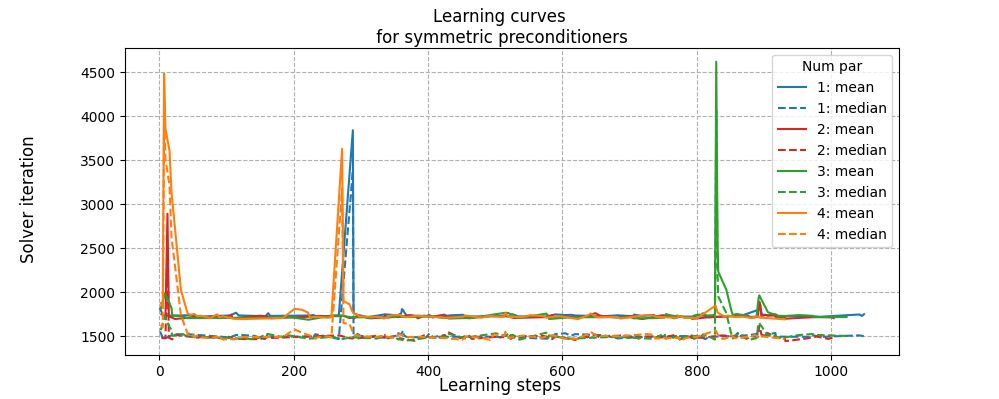
\includegraphics[width=\textwidth]{plots/sym_super_sub_learn_curve.png}
    \caption{Learning curves for from the learning of symmetric preconditioners with 1 super- and subdiagonal. WIth colour corresponding to a different number of partitions and linestyle to mean or median solver iteration count.}
    \label{fig: sym super sub learning curves}
\end{figure}

On major difference in the learning for all of the runs is the actual 
+run time of each of the configurations. When compared with the similar test of section \ref{sec: super sub} it has increased significantly. The cause of the increase in run time is that changes made to the preconditioners during learning increased the solver iteration counts significantly of most of the systems and therefore some of the learning steps takes significantly longer than other. An example can be seen as the spikes in figure \ref{fig: sym super sub learning curves} where such a state was accept. The cause of large increase in solver iteration count because the change made to a coefficient has a larger affect on the preconditioners. A solution would entail a change in the distribution generating the changes made to the coefficients, but changes to this distribution would also have effects on the learning time. With this being the only major difference in the learning of the preconditioner.

In the evaluation of the learned preconditioners, figure \ref{fig: sym super sub test measure} and \ref{fig: sym super sub BvJ}, there is only marginal differences between the solver iteration counts of these tests and the test with unsymmetric preconditioners in section \ref{sec: super sub} seed 0. Because of the increase in run time of the learning algorithm we conclude that using a the symmetric variant of out preconditioner bad.

\begin{figure}[H]
    \center
    \begin{minipage}{.49\textwidth}
        \center
        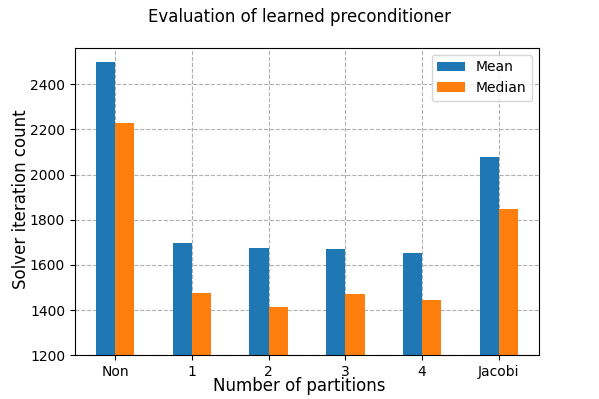
\includegraphics[width=1\textwidth]{plots/sym_super_sub_test_measure.png}
        \caption{Mean (blue) and median (orange) solver iteration counts from the evaluation of the learned preconditioners, with unpreconditioned and Jacobi preconditioning for comparison.}
        \label{fig: sym super sub test measure}
    \end{minipage}
    \begin{minipage}{.02\textwidth}
        
    \end{minipage}
    \begin{minipage}{.49\textwidth}
        \center
        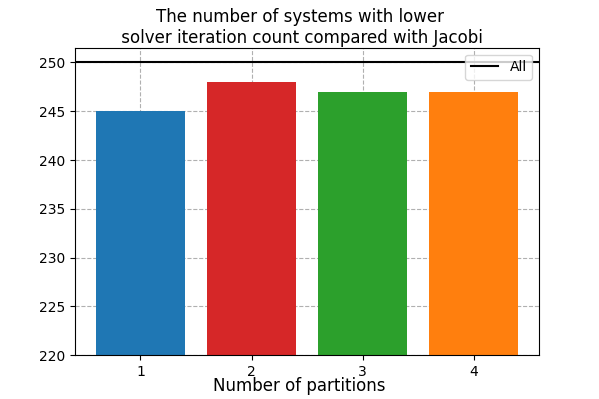
\includegraphics[width=1\textwidth]{plots/sym_super_sub_BvJ.png}
        \caption{Bar graph showing how many individual systems that has a lower solver iteration count with the learned preconditioners compared with its Jacobi preconditioned counterpart.}
        \label{fig: sym super sub BvJ}
    \end{minipage}
\end{figure}


